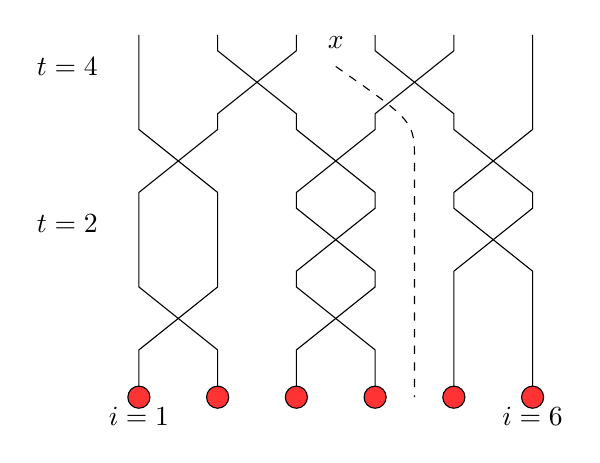
\begin{tikzpicture}[scale = 1]
\draw (0,0) node[below]{$i=1$} -- (0,.6) -- (1,1.4) -- (1,2.6) -- (0,3.4) -- (0,4.6);
\filldraw[color=black, fill=red!80] (0,0) circle (4pt) node[anchor=west] { };
\draw (1,0) -- (1,.6) -- (0,1.4) -- (0,2.6) -- (1,3.4) -- (1,3.6) -- (2,4.4) -- (2,4.6);
\filldraw[color=black, fill=red!80] (1,0) circle (4pt) node[anchor=west] { };
\draw (2,0) -- (2,.6) -- (3,1.4) -- (3,1.6) -- (2,2.4) -- (2,2.6) -- (3,3.4) -- (3,3.6) -- (4,4.4) -- (4,4.6);
\filldraw[color=black, fill=red!80] (2,0) circle (4pt) node[anchor=west] { };
\draw (3,0) -- (3,.6) -- (2,1.4) -- (2,1.6) -- (3,2.4) -- (3,2.6) -- (2,3.4) -- (2,3.6) -- (1,4.4) -- (1,4.6);
\filldraw[color=black, fill=red!80] (3,0) circle (4pt) node[anchor=west] { };
\draw (4,0) -- (4,1.6) -- (5,2.4) -- (5,2.6) -- (4,3.4) -- (4,3.6) -- (3,4.4) -- (3,4.6);
\filldraw[color=black, fill=red!80] (4,0) circle (4pt) node[anchor=west] { };
\draw (5,0) node[below]{$i=6$} -- (5,1.6) -- (4,2.4) -- (4,2.6) -- (5,3.4) -- (5,4.6);
\filldraw[color=black, fill=red!80] (5,0) circle (4pt) node[anchor=west] { };



\draw[fill=blue!50] (-.4,2.2) node[left] {$t=2$};
\draw[fill=blue!50] (-.4,4.2) node[left] {$t=4$};

\draw (2.5,4.5) node{$x$};
\draw [dashed] (2.5,4.2) .. controls (3.5,3.5) .. (3.5,3) 
                         .. controls (3.5,1.5) .. (3.5,1) 
                         .. controls (3.5,0.5) .. (3.5,0.5) 
                         .. controls (3.5,0.0) .. (3.5,0);
\end{tikzpicture}